\documentclass[conference]{IEEEtran}
\usepackage{cite}
\usepackage{amsmath,amssymb,amsfonts}
\usepackage{parskip}
\usepackage{algorithmic}
\usepackage{graphicx}
\usepackage{float}
\usepackage{textcomp}
\usepackage{xcolor}
\usepackage[english]{babel}
\usepackage[utf8x]{inputenc}
\usepackage[T1]{fontenc}
\usepackage[a4paper,top=3cm,bottom=2cm,left=3cm,right=3cm,marginparwidth=1.75cm]{geometry}
\setlength {\marginparwidth }{2cm}
\usepackage[colorinlistoftodos]{todonotes}
\usepackage[colorlinks=true, allcolors=blue]{hyperref}
\def\BibTeX{{\rm B\kern-.05em{\sc i\kern-.025em b}\kern-.08em T\kern-.1667em\lower.7ex\hbox{E}\kern-.125emX}}

\begin{document}
\title{Advancements in Computer Architecture through the use of Machine Learning\\
    \author{
        \IEEEauthorblockN{Edward Nafornita}
        \IEEEauthorblockA{\textit{Department of Computer Science} \\
            \textit{February 27\textsuperscript{th} 2023}\\ 
            Tecumseh, Canada \\
            ID: 110076381 \\ 
            naforni@uwindsor.ca
        }
    }
}
% Create the cover page and the main title on the document
\begin{titlepage}

    \newcommand{\HRule}{\rule{\linewidth}{0.5mm}} % Defines a new command for the horizontal lines, change thickness here
    
    %----------------------------------------------------------------------------------------
    %	LOGO SECTION
    %----------------------------------------------------------------------------------------
    \centering
    
\includegraphics[width=8cm]{title/logo.jpg}\\[1cm] % Include a department/university logo - this will require the graphicx package
     
    %----------------------------------------------------------------------------------------
    
    \center % Center everything on the page
    
    %----------------------------------------------------------------------------------------
    %	HEADING SECTIONS
    %----------------------------------------------------------------------------------------
    
    \textsc{\LARGE Technical Report}\\[1.5cm] 
    \textsc{\Large COMP-2660}\\[0.5cm] 
    \textsc{\large Computer Architecture II}\\[0.5cm] 
    
    %----------------------------------------------------------------------------------------
    %	TITLE SECTION
    %----------------------------------------------------------------------------------------
    \makeatletter
    \HRule \\[0.4cm]
    { \huge \bfseries Advancements in Computer Architecture through the use of Machine Learning}\\[0.4cm] % Title of your document
    \HRule \\[1.5cm]
     
    %----------------------------------------------------------------------------------------
    %	AUTHOR SECTION
    %----------------------------------------------------------------------------------------
    
    \begin{minipage}{0.4\textwidth}
    \begin{flushleft} \large
    \emph{Author:}\\
    Edward Nafornita \\ 
    Student ID: 110076381
    \end{flushleft}
    \end{minipage}
    ~
    \begin{minipage}{0.4\textwidth}
    \begin{flushright} \large
    \emph{Submitted to:} \\
    Reem Al-Saidi \\[1.2em] 
    \end{flushright}
    \end{minipage}\\[2cm]
    \makeatother
    
    %----------------------------------------------------------------------------------------
    %	DATE SECTION
    %----------------------------------------------------------------------------------------
    
    {\large February 27\textsuperscript{th} 2023}\\[2cm]
    
    ``I confirm that I will keep the content of this assignment confidential. I confirm that I have not received any unauthorized 
    assistance in preparing for or writing this assignment. I acknowledge that a mark of zero may be assigned for copied work.''
    \vfill % Fill the rest of the page with whitespace
    \end{titlepage}
\maketitle

\section{Introduction}
Computer architecture has become increasingly complex in recent years, with more and more components 
and layers added to improve performance, power efficiency, and functionality. As a result, designing 
computer architecture has become a challenging task that requires a great deal of expertise, time, 
and resources. Machine learning (ML), a field of artificial intelligence (AI), has emerged as a powerful tool for 
optimising computer architecture by predicting system performance, reducing power consumption, and improving 
design efficiency. ML algorithms have been applied to various aspects of computer architecture, 
including microarchitecture design, network-on-chip/system-on-chip communication, cache design, memory system design, 
and branch prediction. Microarchitecture design, a field of computer architecture which involves the meticulous 
developmental process of the central processing unit (CPU). Microarchitecture is the process of creating a 
microprocessor. This microprocessor is tailored to complete a set of instructions which will be implemented in the 
CPU, this set of instructions are known as the instruction set architecture (ISA). ISA is the result of combining 
logic gates, small/medium-scale circuitry, and registers to perform various logical operations. The most common 
instruction set architecture is Intel's x86 ISA implementation. It is widely used and taught throughout 
the field of computer science and, specifically, computer architecture courses. The creation of microprocessors to 
compute basic logical operations allows for the creation of greater scaled processors such as the arithmetic logic 
unit and general purpose registers which can be combined to create the CPU. Microarchitecture will always remain 
as the fundamental building blocks of a computer system, however, it is not the only fundamental unit for a computer.
Memory system design is the process of developing a system of clocks and logic gates through the use of microarchitecture.
This design is what is known as system-on-chip (SoC) and is one of the two main methods of determining the transfer speeds of 
the computer. Some of the main memory designs that are used in today's computer architecture include; dynamic random access 
memory (DRAM), static random access memory (SRAM), read-only memory (ROM), and/or embedded dynamic random access memory (eDRAM).
The other method of determining the transfer speeds of the computer is through measuring the speeds of the cache system design.
Cache is small, high-speed memory which is used to improve the performance of the computer by optimising the speed of accessing 
data from the main memory modules. Cache design is an important part of the computer as the larger the available cache in the processor, 
the faster the processor. In computer architecture, the cache system is built directly in the CPU so that the CPU may have access to memory 
locally creating an efficient way to resolve quick logical operations. Otherwise, the CPU would have to access memory in the form of 
random access memory (RAM) which is inefficient when compared to cache. Furthermore, network-on-chip (NoC) communication allows for 
communication between multiple cores in the system's processor. This is beneficial as the processor will have the capability to 
dedicate the cores to various processes which will expediate the computational time of the task requested from the CPU. 
Network-on-chip is a key component when looking towards future development of computer architecture as it introduces the topic of 
multiprocessing and multi-threading. When it comes to computer architecture, network-on-chip is a topic which benefits from the research of 
ML for optimisation of power consumption and efficiency of process handling. With regards to network-on-chip communication, branch prediction 
is a fundamental concept in computer architecture which benefits from the high-efficiency performance model for NoC communication. Branch prediction 
refers to the choices that the processor has to compute when prompted, and thus, branch prediction is an efficiency model to expediate the 
choices made by the processor by predicting the best choice of action for series of instructions it was prompted with. This provides the processor with a further boost to performance. 
Evidently, these topics in the field of computer architecture can combine the revolutionary discovery of artificial intelligence and machine learning 
to provide more efficient architecture. Throughout this article, we will explore the applications of ML in computer architecture, the challenges 
associated with its implementation, and future research directions in the field.

\section{Importance}
Machine learning is becoming increasingly important in computer architecture due to its ability to optimise performance, energy efficiency, and reliability. 
Seen throughout the industry for processor manufacturing, machine learning has become a staple in chip design as without the help of ML it takes large teams of 
experts to configure and refine the designs of the CPU. With the help of machine learning, not only does it reduce the cost of manufacturing limiting
human error, but also allots the large team of experts more time to help in the overall design of the architecture. That way manufacturing companies can 
be more efficient when designing chips and they can follow through the design plan, which was also precisely structured through machine learning, knowing that 
the drafts of the architecture are functional and can operate at the precedented level of performance expected in this era. Overall, ML has been seen as a valuable 
tool in the field of computer architecture as it provides a more efficient, cost effective and convenient way of creating and implementing theoretical computer 
architectures into physical components used in this era's computer systems.

\section{Technological Details} % if split 50/50 for section 3 & 4 this will be 692 words and section 4 will be 691
Machine learning in computer architecture involves the use of various techniques which involve the use of advanced algorithms and models to optimise the 
performance of computer systems. For example, a key application for machine learning in computer architecture is the optimisation of SoC designs. SoCs are 
complex circuits that combine multiple components such as processors, memory, and input/output devices (I/O devices), onto a single chip. Machine learning can 
prove to be a useful tool when configuring the ideal design of this chip. This will be done through the analysis of various other methods of implementation of SoCs 
and choosing the best parts of each method. With these fragments of each design, the machine learning algorithm can create a draft of the design that experts may 
analyse and verify the integrity of the design. If the design is valid, experts will move into the next phase of physically creating the chip. From there, the chip 
will be put under various tests to see how it performs in comparison to the test the algorithm searched through. This is a generic flow of how machine learning can 
be applicable to chip design. SoCs are not the only chip that expert manufacturers continuously research and redesign. Topics such as power management are also viewed 
as areas that can be improved upon. Machine learning can use the vast amount of data available both from internal testing (testing that is done at the manufacturer) and 
external testing (testing that is done by consumers) to view what the baseline power consumption rating is for the most current chip used by consumers. From there, the 
algorithm can improve on the design of various components in systems to attempt to reduce the power consumption by them. Such components like the motherboard, the CPU,
RAM, and most significantly, the power supply unit, are such components which are considered when attempting to improve power consumption. 
For example, Figure 1 shows the power consumption of Intel CPUs with different numbers of cores present in the CPU from a study performed by Totoni et al. (2012). Notice how the more the cores present the more the 
power draw is for each CPU. The use of machine learning attempts to minimise the growth of power draw for new CPUs however still ensuring they provide an increase in performance 
when compared to previous year's architecture.
\begin{figure}[H]
    \centering
    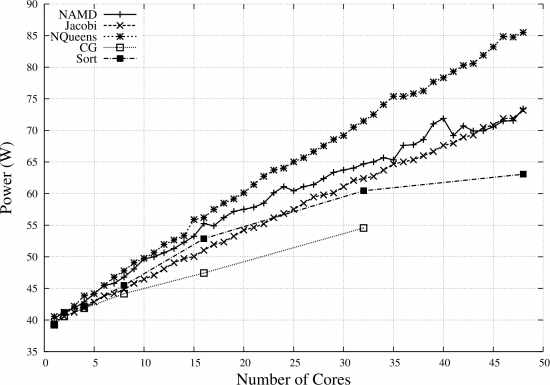
\includegraphics[width=7.2cm]{imgs/powerconsumption-cpu.png}
    \caption{\textit{Intel Core i7 processors with various numbers of cores and their respective power consumption values.} [2]}  
    \label{fig:picture}
\end{figure}

In addition to SoCs, network-on-chip communication is another field which benefits from machine learning. Originally communication inside a processor was integrated through transferring singals between 
the various cores. However, as of more recent development, network-on-chip communication was established and created a more efficient model of communication inside the processor. NoCs use 
data packets rather than signals for communication. Machine learning has been introduced to the NoC architecture as it has been found to reduce the transfer latency of the data packets. 
This, however, required a new variation of the original NoC called the machine learning NoC (M/L NoC). M/L NoC has seen vast improvements over the original NoC architecture especially through the dynamic 
voltage and frequency scaling (DVFS) management for NoCs. DVFS research mostly consisted of reducing dynamic energy consumption at runtime, which essentially means reducing power consumption that occurs 
when the processor is actively running. However, as of recent a recent study performed by Quintin Fettes et al. (2019), their goal was to reduce the static energy build up as a result of the decrease in 
size of transistors. Fetts et al. proposed the hypothesis that, ``an optimal DVFS algorithm should operate at the lowest supply voltage allowable without causing significant performance degradation.''
They created a machine learning algorithm known as ``Learning-enabled Energy-Aware Dynamic voltage/frequency scaling'' or LEAD for short. This algorithm performed exceptionally well and saved approximately 
15 percent in energy savings with only approximately 1 percent in the throughput measurement, which is hardly noticeable when analysing latency. Figure 3 shows an analysis performed by Fettes et al. comparing 
throughput (number of units that can be produced by a production process within a certain period of time [9]) to the dynamic energy savings across various thresholds of utilisation. This provides a perfect example 
of how an algorithm can implement machine learning to adjust various values to conserve power whilst also ensuring little to no performance hinderance, [5], [7].
\begin{figure}
    \centering
    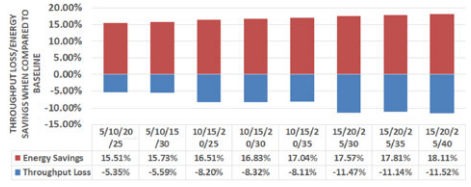
\includegraphics[width=7.2cm]{imgs/dvfs-LEAD-savings.png}
    \caption{\textit{Throughput loss/dynamic energy savings across multiple thresholds sections trace with a window size of 100} [7]}
\end{figure}

Another area of research in machine learning for computer architecture is the optimisation of branch prediction. This component of the CPU is fundamental amongst 
the vast majority of modern processors. Algorithms which are used by machine learning analyse the history of branch instructions and formulate predictions for future branches. 
The study in this field of research is targetted at reducing the number of mispredictions that the algorithm produces. If experts can train the algorithm to catch more of these 
mispredictions, the processor will have a higher efficiency rating in branch prediction thus increasing the overall performance of the processor.
Figure 3 is provided to explain what branch prediction would look like in a visual manner. As stated before, machine learning will make minor tweaks to increase the overall accuracy 
of the prediction algorithm.
\begin{figure}[H]
    \centering
    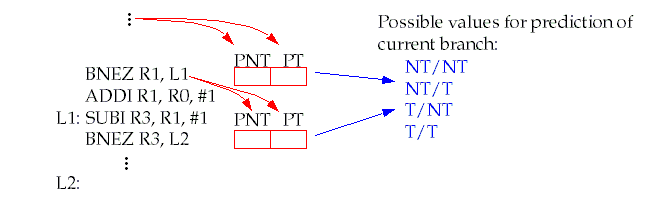
\includegraphics[width=7.2cm]{imgs/branch-prediction.png}
    \caption{\textit{Branch prediction algorithm to predict the conditional statement choice.} [4]}
    \label{fig3:picture}
\end{figure}

\section{Discussion}
The various examples elaborated on are only a small fraction of the total number of applications for machine learning in computer architecture. Evidently, the usage of ML in computer 
architecture has allowed manufacturers, experts, technical designers, and ultimately consumers to benefit from processors which are responsive and reliable. Machine learning has come a 
long way since its first introduction into the computer science field. The difficulties with its implementation normally come from a poor understanding of the theoretical aspects in ML. 
In general, the idea of ML is that you have an algorithm which can learn from past iterations of its lifespan. This repetition will train the algorithm and through multiple iterations 
it will be able to calculate a percentage of its accuracy in a certain task. This is what is known as a neural network, a series of events with lifespans which trains the algorithm to 
learn what are the optimal output values or what the expected results are for that algorithm. As an idea, machine learning seems self-explanatory, however the issues arise when you have 
to apply the algorithm to a very specific task such as in the computer architecture field. The components you work with in the developmental processes of computer architecture are very 
miniscule. Thus, any slight variations to the algorithm and the data that you have collected from the training process of the algorithm will cause unwanted results. These results can 
very from small scale issues, to very costly large scale logical errors. Leaving the whole developmental process up to machine learning is something that we haven't done as of yet due 
to the nature of the concept being a wildcard. The future outlook for machine learning as of right now is to be only a tool in computer architecture and other various fields as it is 
best to let expert manufacturers or technical designers do what they do best. It would be much simplier to correct a human error than a logical error that was overlooked in a machine 
learning algorithm. However, in the current implementations that machine learning has been used in, it has conquored great feats for technological advancements. The small form factor 
of today's microarchitecture causes a plethora of problems for human modifications. Although, through the very intricate analysis of machine learning, experts have fabricated 
processors which are able to withstand large amounts of data transfers, quickly and effectively perform logical operations, and reduce the overall cost of mass-producing the chips in 
today's market. As a further future outlook, I find the use of machine learning as a vital tool when working with very low level programming. With the help of ML, assembly programming 
will be able to be the most optimised method of creating a program which can solve very specific tasks with incredible performance and accuracy. Additionally, with the help of ML, 
computer architecture may eventually solve some of the most common problems when it comes to reducing costs of microprocessors. The current issues that are hindering the abilities of chip 
manufacturers is due to undesired quantum tunneling when working with CPU architecture on the scales of one nanometer to four nanometers. This may be a technological advancement that may 
be solved through the use of machine learning. 

\section{Conclusion} 
In conclusion, machine learning is a rapidly growing field with significant potential for optimising computer architecture. Advanced algorithms and models have shown to the technological 
world that it is possible to design computer systems that are tailored to specific requirements such as performance, power consumption, and reliability. The use of ML in computer architecture 
has already led to several innovative applications. Some of which include; optimised system-on-chip/network-on-chip designs and communication, power management through the LEAD algorithm, 
and memory systems. However, there are multiple challenges associated with the use of machine learning. The largest limitation for machine learning is that it requires large datasets and 
computational resources, as well as the potential risks and the other limitations of different machine learning algorithms and models. As this field of computer architectural design continues 
to evolve, it will become quite imperative to carefully balance the potential benefits of ML with the need to ensure the safety, reliability and security components of computer systems. Furthermore, 
machine learning has shown the capability of automation for the industry of chip manufacturers, efficiently creating and optimising microchips. One such example mentioned before was through the 
LEAD algorithm which showed how a properly trained artificial intelligence algorithm can single handedly increase the performance modern day computer systems. Overall, the use of machine learning 
in computer architecture represents a promising approach for designing and optimising computer systems in the era of big data and complex applications such as artificial intelligence.

\begin{thebibliography}{00}
    \bibitem{b1} ``Computer System Designs: System-on-chip,'' O'Reilly Online Learning. [Online]. Available: \url{https://www.oreilly.com/library/view/computer-system-designs/9780470643365/c04.xhtml}.
    \bibitem{b2} E. Totoni, B. Behzad, S. Ghike and J. Torrellas, ``Comparing the power and performance of Intel's SCC to state-of-the-art CPUs and GPUs,'' 2012 IEEE International Symposium on Performance Analysis of Systems \& Software, New Brunswick, NJ, USA, 2012, pp. 78-87, doi: 10.1109/ISPASS.2012.6189208.
    \bibitem{b3} J. Dean, ``1.1 The Deep Learning Revolution and Its Implications for Computer Architecture and Chip Design,'' 2020 IEEE International Solid-State Circuits Conference - (ISSCC), San Francisco, CA, USA, 2020, pp. 8-14, doi: 10.1109/ISSCC19947.2020.9063049.
    \bibitem{b4} J. Plusquellic, ``Dynamic Branch Prediction,'' Advanced Computer Architecture. [Online]. Available: \url{http://ece-research.unm.edu/jimp/611/slides/chap4_5.html}.
    \bibitem{b5} K. Balamurugan, ``Roadmap for machine learning based network-on-chip (M/L NoC) technology and its analysis for researchers,'' Institute of Physics [Online]. Available: \url{https://iopscience.iop.org/article/10.1088/2399-6528/ac4dd5}. 
    \bibitem{b6} ``Principles of Cache Design - technical articles,'' All About Circuits. [Online]. Available: \url{https://www.allaboutcircuits.com/technical-articles/principles-of-cache-design/}.
    \bibitem{b7} Q. Fettes, M. Clark, R. Bunescu, A. Karanth, and A. Louri, ``Dynamic voltage and frequency scaling in nocs with supervised and Reinforcement Learning Techniques,'' Mar-2019. [Online]. Available: \url{https://ieeexplore.ieee.org/document/8489913}. 
    \bibitem{b8} ``What is Microarchitecture (µarch)? - definition from Techopedia,'' Techopedia.com. [Online]. Available: \url{https://www.techopedia.com/definition/4502/microarchitecture-arch}.
    \bibitem{b9} ``What is network on a chip (NOC)? - definition from Techopedia,'' Techopedia.com. [Online]. Available: \url{https://www.techopedia.com/definition/30647/network-on-a-chip-noc}.
    \bibitem{b10} ``What is throughput? - definition from Techopedia,'' Techopedia.com. [Online]. Available: \url{https://www.techopedia.com/definition/5573/throughput}. 
\end{thebibliography}
\end{document}
